\documentclass{standalone}
\usepackage{tikz}
\usetikzlibrary{positioning}
\usetikzlibrary {shapes.geometric}
\usetikzlibrary {backgrounds}
\usetikzlibrary {calc}

\tikzstyle{lOneBlock} = [circle, draw, fill=lightgray, inner sep=2]
\tikzstyle{lOneTx} = [rectangle, minimum width=1cm, minimum height = 0.1cm, inner sep=0, outer sep=0]
\tikzstyle{lTwoTx} = [rectangle, \rollupColor, minimum width=0.4cm, minimum height = 0.1cm, inner sep=0, outer sep=0]
\tikzstyle{background rectangle} = [fill=white]


\newcommand{\timeline}{
    \node (t0) at (0,0) {};
    \node (tEnd) at (10,0) {};
    \draw (t0) [->, thick]  -- (tEnd);
    \foreach \idx in {0,...,2}{
        \node (lOneBlock\idx) [lOneBlock] at (1 + \idx * 4, 0) {};
    };
}

\newcommand{\lOneTransactions}{
    \foreach \blockIdx in {0,...,2}{
        \node (txPos) at (0, 1) {};
        \foreach \txIdx in {0,...,5} {
            \node[draw, lOneTx, anchor=north] (tx-\blockIdx-\txIdx) at (lOneBlock\blockIdx |- txPos) {};
            \node (txPos) at (tx-\blockIdx-\txIdx.south) {};
        }
    };
    \node[yshift=0.1cm, anchor=south] at (tx-0-0.north) {\tiny \texttt{Block x-2}};
    \node[yshift=0.1cm, anchor=south] at (tx-1-0.north) {\tiny \texttt{Block x-1}};
    \node[yshift=0.1cm, anchor=south] at (tx-2-0.north) {\tiny \texttt{Block x}};
}

\begin{document}

% Introduce L1 chain
\ifnum \sourceNo = 0
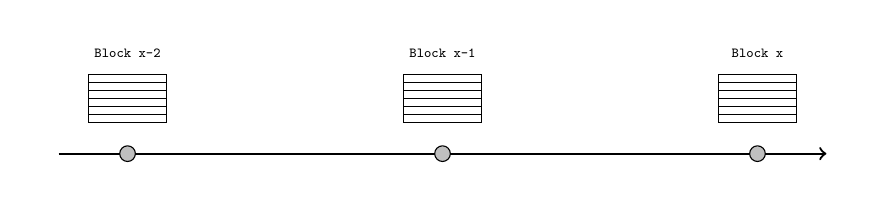
\begin{tikzpicture}[framed]
    \timeline
    \lOneTransactions
\end{tikzpicture}
\fi

% Instead of passing parameters to the diagram commands, define them as variables
% This makes it easier to reuse variables between different diagrams and also makes the diagram commands more readable
\newcommand{\anchorBlockNum}{1}
\newcommand{\numLTwoBlocks}{6}
\newcommand{\rollupName}{A}
\newcommand{\rollupColor}{blue}
\newcommand{\rollupOffset}{-0.3cm}
\newcommand{\pubTx}{tx-2-3}
\newcommand{\anchorBlock}{lOneBlock\anchorBlockNum}
\newcommand{\anchorColor}{magenta}


\newcommand{\lTwoTransactions}{
    \node[yshift=\rollupOffset, xshift=0.5cm] (blockPos) at (\anchorBlock) {};
    \foreach \idx in {0,...,\numLTwoBlocks}{
        \node (lTwoBlock\idx)  at (blockPos) {};
        \node (blockPos) at (blockPos)[xshift=0.5cm] {};
    };

    \foreach \blockIdx in {0,...,\numLTwoBlocks} {
        \node (txPos) at (lTwoBlock\blockIdx) {};
        \foreach \txIdx in {0,...,4}{
            \node[draw, lTwoTx, anchor=north] (l2Tx-\rollupName-\blockIdx-\txIdx) at (txPos) {};
            \node (txPos) at (l2Tx-\rollupName-\blockIdx-\txIdx.south) {};
        }
    }
}


% Usage: \partialPublication{startBlock}{endBlock}
\newcommand{\partialPublication}[2]{
    \node[draw, lOneTx, fill=\rollupColor] at (\pubTx) {};
    \node[xshift=-0.1cm, yshift=0.1cm] (topLeft) at (l2Tx-\rollupName-#1-0.north west) {};
    \node[xshift=0.1cm, yshift=-0.1cm] (bottomRight) at (l2Tx-\rollupName-#2-4.south east) {};
    \draw[inner sep=0, outer sep=0, rounded corners, \rollupColor] (topLeft) rectangle (bottomRight) {};
    \node[inner sep=0, outer sep=0] (top) at ($(topLeft)!0.5!(bottomRight |- topLeft)$) {};
    \draw[inner sep=0, outer sep=0, ->, \rollupColor] (top) to[in=180] (\pubTx.west);
}
\newcommand{\publication}{\partialPublication{0}{\numLTwoBlocks}}

% Introduce L2 chain
\ifnum \sourceNo = 1
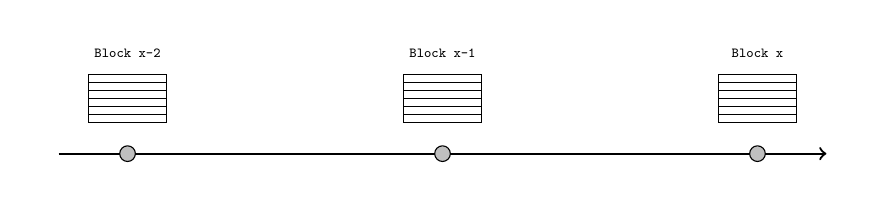
\begin{tikzpicture}[framed]
    \timeline
    \lOneTransactions
    \lTwoTransactions
    \publication
\end{tikzpicture}
\fi

% L2 publications may span multiple L1 slots
\renewcommand{\anchorBlockNum}{0}
\renewcommand{\numLTwoBlocks}{14}

\ifnum \sourceNo = 2
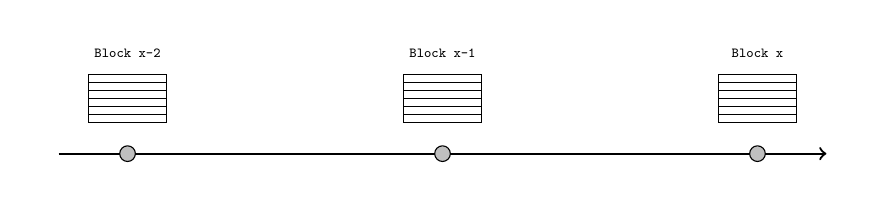
\begin{tikzpicture}[framed]
    \timeline
    \lOneTransactions
    \lTwoTransactions
    \publication
\end{tikzpicture}
\fi

\newcommand{\snapshotAt}[1]{
    \node (top) at (#1, 1.5) {};
    \node (bottom) at (#1, -1) {};

    \fill [fill=white, opacity=0.7] (top) rectangle (tEnd |- bottom);
    \clip (t0 |- top) rectangle (bottom);
}

\newcommand{\injectAnchorToBlock}[1]{
    \node[draw, lOneBlock, fill=\anchorColor] at (\anchorBlock) {};
    \node[draw, lTwoTx, fill=\anchorColor, minimum width=0.1cm, anchor=west] at (l2Tx-\rollupName-#1-0.west) {};
    \draw[->, \anchorColor] (\anchorBlock.south) to[bend right] (l2Tx-\rollupName-#1-0.west);
}
\newcommand{\injectAnchor}{\injectAnchorToBlock{0}}

% Snapshot after L2 transaction
\ifnum \sourceNo = 3
\begin{tikzpicture}[framed]
    \timeline

    \snapshotAt{4.25}
    
    \lOneTransactions
    \lTwoTransactions
    \injectAnchor

    \node[draw, lOneTx, fill=teal] at (tx-0-4) {};
    \node[draw, lTwoTx, fill=green] at (l2Tx-A-1-2) {};
\end{tikzpicture}
\fi

\newcommand{\validateAnchor}{
    \node[draw, lOneTx, fill=\anchorColor, minimum width=0.1cm, anchor=west] (anchorValidation) at (\pubTx.west) {};
    \draw[->, \anchorColor] (\anchorBlock.north east) to[bend left] (anchorValidation.west);
}

% Anchor block hash is validated
\ifnum \sourceNo = 4
\begin{tikzpicture}[framed]
    \timeline

    \lOneTransactions
    \lTwoTransactions
    \publication
    \injectAnchor
    \validateAnchor

    \node[draw, lOneTx, fill=teal] at (tx-0-4) {};
    \node[draw, lTwoTx, fill=green] at (l2Tx-A-1-2) {};

\end{tikzpicture}
\fi

% Same Slot Assertion
\ifnum \sourceNo = 5
\begin{tikzpicture}[framed]
    \timeline

    \lOneTransactions
    \lTwoTransactions
    \publication
    
    \node[draw, lOneTx, fill=orange] at (tx-2-1) {};
    \node[draw, lTwoTx, fill=orange, minimum width=0.1cm, anchor=west] (assertion) at (l2Tx-A-9-0.west) {};
    \draw[->, orange] (tx-2-1.west) to[bend right] (assertion.north);

    \node[draw, lTwoTx, fill=green] at (l2Tx-A-9-2) {};
\end{tikzpicture}
\fi

% Multiple anchor blocks
\ifnum \sourceNo = 6
\begin{tikzpicture}[framed]
    \timeline

    \lOneTransactions
    \lTwoTransactions
    \publication
    \injectAnchor

    \renewcommand{\anchorBlockNum}{1}
    \renewcommand{\anchorColor}{brown}
    \injectAnchorToBlock{8}
    \validateAnchor
    
    \node[draw, lOneTx, fill=teal] at (tx-1-4) {};
    \node[draw, lTwoTx, fill=green] at (l2Tx-A-8-2) {};
\end{tikzpicture}
\fi


% Interdependent L2 transactions
\ifnum \sourceNo = 7
\begin{tikzpicture}[framed]
    \timeline

    \snapshotAt{4.25}

    \lOneTransactions
    \lTwoTransactions

    \node[draw, lTwoTx, fill=green] at (l2Tx-A-1-3) {};
    \node[draw, lTwoTx, fill=olive] at (l2Tx-A-3-1) {};
    \node[draw, lTwoTx, fill=olive, minimum width=0.1cm, anchor=west] (assertion) at (l2Tx-A-1-2.west) {};
    \draw[->, olive] (l2Tx-A-3-1.west) to[bend right] (assertion);
\end{tikzpicture}
\fi

% Cross rollup atomicity
\ifnum \sourceNo = 8
\begin{tikzpicture}[framed]
    \timeline

    \lOneTransactions
    \lTwoTransactions
    \publication
    \node[draw, lTwoTx, fill=cyan] at (l2Tx-A-1-3) {};
    \node[draw, lTwoTx, fill=violet, minimum width=0.1cm, anchor=west] (assertionA) at (l2Tx-A-1-1.west) {};


    \renewcommand{\rollupName}{B}
    \renewcommand{\rollupColor}{brown}
    \renewcommand{\rollupOffset}{-1.1cm}
    \renewcommand{\pubTx}{tx-2-4}
    
    \lTwoTransactions
    \publication
    \node[draw, lTwoTx, fill=violet] at (l2Tx-B-5-1) {};
    \node[draw, lTwoTx, fill=cyan, minimum width=0.1cm, anchor=west] (assertionB) at (l2Tx-B-3-3.west) {};

    \draw[->, violet] (l2Tx-B-5-1.north) to[bend right] (assertionA.east);
    \draw[->, cyan] (l2Tx-A-1-3.south) to[bend right] (assertionB.west);


\end{tikzpicture}
\fi

% Sub-publication proof
\ifnum \sourceNo = 9
\begin{tikzpicture}[framed]
    \timeline
    \lOneTransactions
    \lTwoTransactions
    % The first partial publication overlaps with L2 block 5. I will remove that block for clarity
    % There is probably an intelligent way to do this using \clip but I will just overwrite it
    \node[xshift=-0.05cm, yshift=0.05cm] (topLeft) at (l2Tx-A-5-0.north west) {};
    \node[xshift=0.05cm, yshift=-0.05cm] (bottomRight) at (l2Tx-A-5-4.south east) {};
    \fill[white] (topLeft) rectangle (bottomRight);

    \partialPublication{0}{4}
    \renewcommand{\pubTx}{tx-2-4}
    \partialPublication{6}{\numLTwoBlocks}

\end{tikzpicture}
\fi


% A collection of assertions
\ifnum \sourceNo = 10
\begin{tikzpicture}[framed]
    \timeline

    \snapshotAt{7.25}
    
    \lOneTransactions
    \lTwoTransactions

    \foreach \block/\tx in {1/2, 3/3, 4/2, 4/4, 7/1, 10/3} {
        \node[draw, lTwoTx, fill=magenta] at (l2Tx-A-\block-\tx) {};
    }
    
\end{tikzpicture}
\fi

% The end-of-publication assertion
\ifnum \sourceNo = 11
\begin{tikzpicture}[framed]
    \timeline

    \lOneTransactions
    \lTwoTransactions

    \foreach \block/\tx in {1/2, 3/3, 4/2, 4/4, 7/1, 10/3} {
        \node[draw, lTwoTx, fill=magenta] at (l2Tx-A-\block-\tx) {};
    }
    

    \node[draw, lTwoTx, fill=gray] (finalBlock) at (l2Tx-A-\numLTwoBlocks-4) {};
    \publication

    \newcommand{\artifactColor}{orange}
    \node[draw, lTwoTx, fill=\artifactColor, minimum width=0.1cm, anchor=west] (injected) at (finalBlock.west) {};
    \node[draw, lOneTx, fill=\artifactColor, minimum width=0.1cm, anchor=east] (computed) at (\pubTx.east) {};
    \draw[->, \artifactColor] (computed) to[out=270, in=90] (injected);
\end{tikzpicture}
\fi


\end{document}



        